\title{2020 年高考数学 全国III卷-理科}
\date{}
\maketitle

\section*{一、选择题}
本题共12小题，每小题5分，共60分。在每小题给出的四个选项中，只有一项是符合题目要求的。

\begin{question}[points=5]
已知集合 $A=\{(x,y)\mid x,y\in\mathbb{N}^*,\ y\ge x\}$，$B=\{(x,y)\mid x+y=8\}$，则 $A\cap B$ 中元素的个数为
\begin{choices}
  \item $2$
  \item $3$
  \item $4$
  \item $6$
\end{choices}
\begin{solution}
\textbf{答案：}$C$

\textbf{分析：}采用列举法列举出 $A\cap B$ 中元素即可。

\textbf{详解：}由题意，$A\cap B$ 中的元素满足 $\begin{cases} y\ge x \\ x+y=8 \end{cases}$，且 $x,y\in\mathbb{N}^*$，由 $x+y=8\ge 2x$，得 $x\le 4$，所以满足 $x+y=8$ 的有 $(1,7),(2,6),(3,5),(4,4)$，故 $A\cap B$ 中元素的个数为 $4$。故选 $C$。
\end{solution}
\end{question}

\begin{question}[points=5]
复数 $\dfrac{1}{1-3i}$ 的虚部是
\begin{choices}
  \item $-\dfrac{3}{10}$
  \item $-\dfrac{1}{10}$
  \item $\dfrac{1}{10}$
  \item $\dfrac{3}{10}$
\end{choices}
\begin{solution}
\textbf{答案：}$D$

\textbf{分析：}利用复数的除法运算求出 $z$ 即可。

\textbf{详解：}因为 $z=\dfrac{1}{1-3i}=\dfrac{1+3i}{(1-3i)(1+3i)}=\dfrac{1}{10}+\dfrac{3}{10}i$，所以复数 $z=\dfrac{1}{1-3i}$ 的虚部为 $\dfrac{3}{10}$。故选 $D$。
\end{solution}
\end{question}

\begin{question}[points=5]
在一组样本数据中，1,2,3,4 出现的频率分别为 $p_1,p_2,p_3,p_4$，且 $\sum\limits_{i=1}^4 p_i=1$，则下面四种情形中，对应样本的标准差最大的一组是
\begin{choices}
  \item $p_1=p_4=0.1,\ p_2=p_3=0.4$
  \item $p_1=p_4=0.4,\ p_2=p_3=0.1$
  \item $p_1=p_4=0.2,\ p_2=p_3=0.3$
  \item $p_1=p_4=0.3,\ p_2=p_3=0.2$
\end{choices}
\begin{solution}
\textbf{答案：}$B$

\textbf{分析：}计算出四个选项中对应数据的平均数和方差，由此可得出标准差最大的一组。

\textbf{详解：}对于 $A$ 选项，平均数为 $\overline{x}_A=(1+4)\times 0.1+(2+3)\times 0.4=2.5$，方差为 $s_A^2=(1-2.5)^2\times0.1+(2-2.5)^2\times0.4+(3-2.5)^2\times0.4+(4-2.5)^2\times0.1=0.65$。
对于 $B$ 选项，平均数为 $\overline{x}_B=(1+4)\times0.4+(2+3)\times0.1=2.5$，方差为 $s_B^2=(1-2.5)^2\times0.4+(2-2.5)^2\times0.1+(3-2.5)^2\times0.1+(4-2.5)^2\times0.4=1.85$。
对于 $C$ 选项，平均数为 $\overline{x}_C=(1+4)\times0.2+(2+3)\times0.3=2.5$，方差为 $s_C^2=(1-2.5)^2\times0.2+(2-2.5)^2\times0.3+(3-2.5)^2\times0.3+(4-2.5)^2\times0.2=1.05$。
对于 $D$ 选项，平均数为 $\overline{x}_D=(1+4)\times0.3+(2+3)\times0.2=2.5$，方差为 $s_D^2=(1-2.5)^2\times0.3+(2-2.5)^2\times0.2+(3-2.5)^2\times0.2+(4-2.5)^2\times0.3=1.45$。
因此 $B$ 组标准差最大。故选 $B$。
\end{solution}
\end{question}

\begin{question}[points=5]
Logistic 模型是常用数学模型之一，可应用于流行病学领域。有学者根据公布数据建立了某地区新冠肺炎累计确诊病例数 $I(t)$ ($t$ 的单位：天)的 Logistic 模型：$I(t)=\dfrac{K}{1+e^{-0.23(t-53)}}$，其中 $K$ 为最大确诊病例数。当 $I(t^*)=0.95K$ 时，标志着已初步遏制疫情，则 $t^*$ 约为 ($\ln 19\approx 3$)
\begin{choices}
  \item $60$
  \item $63$
  \item $66$
  \item $69$
\end{choices}
\begin{solution}
\textbf{答案：}$C$

\textbf{分析：}将 $t=t^*$ 代入函数 $I(t)=\dfrac{K}{1+e^{-0.23(t-53)}}$ 结合 $I(t^*)=0.95K$ 求得 $t^*$ 即可得解。

\textbf{详解：}因为 $I(t)=\dfrac{K}{1+e^{-0.23(t-53)}}$，所以 $I(t^*)=\dfrac{K}{1+e^{-0.23(t^*-53)}}=0.95K$，则 $e^{0.23(t^*-53)}=19$，所以 $0.23(t^*-53)=\ln 19\approx3$，解得 $t^*\approx\dfrac{3}{0.23}+53\approx66$。故选 $C$。
\end{solution}
\end{question}

\begin{question}[points=5]
设 $O$ 为坐标原点，直线 $x=2$ 与抛物线 $C:y^2=2px(p>0)$ 交于 $D,E$ 两点，若 $OD\perp OE$，则 $C$ 的焦点坐标为
\begin{choices}
  \item $(\dfrac14,0)$
  \item $(\dfrac12,0)$
  \item $(1,0)$
  \item $(2,0)$
\end{choices}
\begin{solution}
\textbf{答案：}$B$

\textbf{分析：}根据 $OD\perp OE$ 结合抛物线的对称性确定 $D$ 点坐标，代入方程求得 $p$，进而求得焦点坐标。

\textbf{详解：}因为直线 $x=2$ 与抛物线 $y^2=2px(p>0)$ 交于 $D,E$ 两点，且 $OD\perp OE$，根据抛物线的对称性可知 $\angle DOx=\angle EO x=\dfrac{\pi}{4}$，所以 $D(2,2)$，代入抛物线方程 $4=4p$，得 $p=1$，所以焦点坐标为 $(\dfrac12,0)$。故选 $B$。
\end{solution}
\end{question}

\begin{question}[points=5]
已知向量 $\mathbf{a},\mathbf{b}$ 满足 $|\mathbf{a}|=5$，$|\mathbf{b}|=6$，$\mathbf{a}\cdot\mathbf{b}=-6$，则 $\cos\langle\mathbf{a},\mathbf{a}+\mathbf{b}\rangle=$
\begin{choices}
  \item $-\dfrac{31}{35}$
  \item $-\dfrac{19}{35}$
  \item $\dfrac{17}{35}$
  \item $\dfrac{19}{35}$
\end{choices}
\begin{solution}
\textbf{答案：}$D$

\textbf{分析：}计算出 $\mathbf{a}\cdot(\mathbf{a}+\mathbf{b})$ 和 $|\mathbf{a}+\mathbf{b}|$ 的值，利用平面向量数量积公式计算。

\textbf{详解：}因为 $|\mathbf{a}|=5$，$|\mathbf{b}|=6$，$\mathbf{a}\cdot\mathbf{b}=-6$，所以 $\mathbf{a}\cdot(\mathbf{a}+\mathbf{b})=|\mathbf{a}|^2+\mathbf{a}\cdot\mathbf{b}=25-6=19$。$|\mathbf{a}+\mathbf{b}|=\sqrt{|\mathbf{a}|^2+2\mathbf{a}\cdot\mathbf{b}+|\mathbf{b}|^2}=\sqrt{25-12+36}=7$。因此 $\cos\langle\mathbf{a},\mathbf{a}+\mathbf{b}\rangle=\dfrac{\mathbf{a}\cdot(\mathbf{a}+\mathbf{b})}{|\mathbf{a}||\mathbf{a}+\mathbf{b}|}=\dfrac{19}{5\times7}=\dfrac{19}{35}$。故选 $D$。
\end{solution}
\end{question}

\begin{question}[points=5]
在 $\triangle ABC$ 中，$\cos C=\dfrac{2}{3}$，$AC=4$，$BC=3$，则 $\cos B=$
\begin{choices}
  \item $\dfrac{1}{9}$
  \item $\dfrac{1}{3}$
  \item $\dfrac{1}{2}$
  \item $\dfrac{2}{3}$
\end{choices}
\begin{solution}
\textbf{答案：}$A$

\textbf{分析：}利用余弦定理先求 $AB$，再利用余弦定理求 $\cos B$。

\textbf{详解：}由余弦定理 $AB^2=AC^2+BC^2-2\cdot AC\cdot BC\cdot\cos C=4^2+3^2-2\times4\times3\times\dfrac{2}{3}=16+9-16=9$，所以 $AB=3$。再由余弦定理 $\cos B=\dfrac{AB^2+BC^2-AC^2}{2\cdot AB\cdot BC}=\dfrac{9+9-16}{2\times3\times3}=\dfrac{2}{18}=\dfrac{1}{9}$。故选 $A$。
\end{solution}
\end{question}

\begin{question}[points=5]
下图为某几何体的三视图，则该几何体的表面积是

\begin{center}
  
\includegraphics[width=.38\linewidth]{question-8-1.jpg}
\end{center}
\begin{choices}
  \item $6+4\sqrt{2}$
  \item $4+4\sqrt{2}$
  \item $6+2\sqrt{3}$
  \item $4+2\sqrt{3}$
\end{choices}
\begin{solution}
\textbf{答案：}$C$

\textbf{分析：}根据三视图特征，在正方体中截取出符合题意的立体图形，求出每个面的面积。

\textbf{详解：}根据三视图特征，在正方体中截取出如图立体图形。$S_{\triangle ABC}=S_{\triangle ADC}=S_{\triangle CDB}=\dfrac12\times2\times2=2$，$AB=AD=DB=2\sqrt{2}$，$\triangle ADB$ 是边长为 $2\sqrt{2}$ 的等边三角形，$S_{\triangle ADB}=\dfrac12\times(2\sqrt{2})^2\times\sin60^\circ=\dfrac12\times8\times\dfrac{\sqrt{3}}{2}=2\sqrt{3}$。所以表面积 $=3\times2+2\sqrt{3}=6+2\sqrt{3}$。故选 $C$。
\end{solution}
\end{question}

\begin{question}[points=5]
已知 $2\tan\theta-\tan\left(\theta+\dfrac{\pi}{4}\right)=7$，则 $\tan\theta=$
\begin{choices}
  \item $-2$
  \item $-1$
  \item $1$
  \item $2$
\end{choices}
\begin{solution}
\textbf{答案：}$D$

\textbf{分析：}利用两角和的正切公式，结合换元法解一元二次方程。

\textbf{详解：}由 $2\tan\theta-\tan(\theta+\frac{\pi}{4})=7$，得 $2\tan\theta-\dfrac{\tan\theta+1}{1-\tan\theta}=7$。令 $t=\tan\theta$，$t\neq1$，则 $2t-\dfrac{t+1}{1-t}=7$，整理得 $t^2-4t+4=0$，解得 $t=2$。所以 $\tan\theta=2$。故选 $D$。
\end{solution}
\end{question}

\begin{question}[points=5]
若直线 $l$ 与曲线 $y=\sqrt{x}$ 和圆 $x^2+y^2=\dfrac{1}{5}$ 都相切，则 $l$ 的方程为
\begin{choices}
  \item $y=2x+1$
  \item $y=2x+\dfrac12$
  \item $y=\dfrac12x+1$
  \item $y=\dfrac12x+\dfrac12$
\end{choices}
\begin{solution}
\textbf{答案：}$D$

\textbf{分析：}设出直线方程，利用导数求切线斜率，利用直线与圆相切列方程求解。

\textbf{详解：}设直线 $l$ 在曲线 $y=\sqrt{x}$ 上的切点为 $(x_0,\sqrt{x_0})$，$x_0>0$。$y'=\dfrac{1}{2\sqrt{x}}$，斜率 $k=\dfrac{1}{2\sqrt{x_0}}$。切线方程为 $y-\sqrt{x_0}=\dfrac{1}{2\sqrt{x_0}}(x-x_0)$，即 $x-2\sqrt{x_0}y+x_0=0$。圆 $x^2+y^2=\dfrac15$ 的圆心为 $(0,0)$，半径 $r=\dfrac{1}{\sqrt{5}}$。由圆心到切线距离等于半径得 $\dfrac{|x_0|}{\sqrt{1+4x_0}}=\dfrac{1}{\sqrt{5}}$，平方得 $5x_0^2=1+4x_0$，即 $5x_0^2-4x_0-1=0$，解得 $x_0=1$（$x_0=-\frac15$ 舍去）。故切线为 $x-2y+1=0$，即 $y=\dfrac12x+\dfrac12$。故选 $D$。
\end{solution}
\end{question}

\begin{question}[points=5]
设双曲线 $C:\dfrac{x^2}{a^2}-\dfrac{y^2}{b^2}=1\ (a>0,b>0)$ 的左、右焦点分别为 $F_1,F_2$，离心率为 $\sqrt{5}$。$P$ 是 $C$ 上一点，且 $F_1P\perp F_2P$。若 $\triangle PF_1F_2$ 的面积为 $4$，则 $a=$
\begin{choices}
  \item $1$
  \item $2$
  \item $4$
  \item $8$
\end{choices}
\begin{solution}
\textbf{答案：}$A$

\textbf{分析：}根据双曲线定义、三角形面积公式、勾股定理，结合离心率公式求解。

\textbf{详解：}因为 $e=\dfrac{c}{a}=\sqrt{5}$，所以 $c=\sqrt{5}a$。根据双曲线定义 $|PF_1|-|PF_2|=2a$。$\triangle PF_1F_2$ 面积 $\dfrac12|PF_1|\cdot|PF_2|=4$，得 $|PF_1|\cdot|PF_2|=8$。又 $F_1P\perp F_2P$，所以 $|PF_1|^2+|PF_2|^2=(2c)^2=20a^2$。而 $(|PF_1|-|PF_2|)^2=4a^2$，即 $|PF_1|^2+|PF_2|^2-2|PF_1|\cdot|PF_2|=4a^2$，所以 $20a^2-16=4a^2$，得 $16a^2=16$，$a=1$。故选 $A$。
\end{solution}
\end{question}

\begin{question}[points=5]
已知 $5^5<8^4$，$13^4<8^5$。设 $a=\log_5 3$，$b=\log_8 5$，$c=\log_{13}8$，则
\begin{choices}
  \item $a<b<c$
  \item $b<a<c$
  \item $b<c<a$
  \item $c<a<b$
\end{choices}
\begin{solution}
\textbf{答案：}$A$

\textbf{分析：}比较 $a,b,c$ 的大小，可先判断范围，再通过作商法、指数式与对数式互化进行比较。

\textbf{详解：}由题意知 $a,b,c\in(0,1)$。$\dfrac{a}{b}=\dfrac{\log_53}{\log_85}=\dfrac{\lg3}{\lg5}\cdot\dfrac{\lg8}{\lg5}<\dfrac{1}{2}\left(\dfrac{\lg3+\lg8}{\lg5}\right)^2=\left(\dfrac{\lg24}{\lg25}\right)^2<1$，所以 $a<b$。由 $b=\log_85$ 得 $8^b=5$，由 $5^5<8^4$ 得 $8^{5b}<8^4$，所以 $5b<4$，$b<\dfrac45$。由 $c=\log_{13}8$ 得 $13^c=8$，由 $13^4<8^5$ 得 $13^4<13^{5c}$，所以 $4<5c$，$c>\dfrac45$。综上 $a<b<c$。故选 $A$。
\end{solution}
\end{question}

\section*{二、填空题}
本题共4小题，每小题5分，共20分。

\begin{question}[points=5]
若 $x,y$ 满足约束条件 $\begin{cases} x+y\ge0 \\ 2x-y\ge0 \\ x\le1 \end{cases}$，则 $z=3x+2y$ 的最大值为 。
\fillin[{$7$}]
\begin{solution}
\textbf{答案：}$7$

\textbf{分析：}作出可行域，利用线性规划求解。

\textbf{详解：}作出可行域如图。由 $z=3x+2y$ 得 $y=-\frac32x+\frac{z}{2}$，当直线经过点 $A$ 时截距最大，$z$ 最大。解 $\begin{cases} y=2x \\ x=1 \end{cases}$ 得 $A(1,2)$，所以 $z_{\max}=3\times1+2\times2=7$。
\end{solution}
\end{question}

\begin{question}[points=5]
$\left(x^2+\dfrac{2}{x}\right)^6$ 的展开式中常数项是 （用数字作答）。
\fillin[{$240$}]
\begin{solution}
\textbf{答案：}$240$

\textbf{分析：}写出二项展开式通项，令 $x$ 的指数为零求得 $r$ 再计算。

\textbf{详解：}$T_{r+1}=C_6^r(x^2)^{6-r}\cdot\left(\dfrac{2}{x}\right)^r=C_6^r 2^r x^{12-3r}$，令 $12-3r=0$，得 $r=4$。常数项为 $C_6^4 2^4=15\times16=240$。
\end{solution}
\end{question}

\begin{question}[points=5]
已知圆锥的底面半径为 $1$，母线长为 $3$，则该圆锥内半径最大的球的体积为 。

\begin{center}
  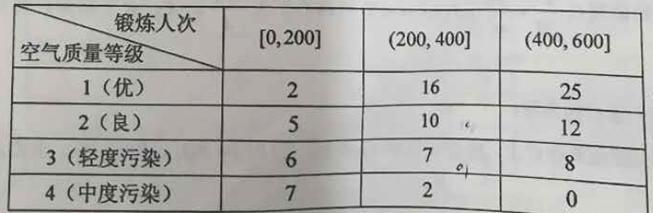
\includegraphics[width=.38\linewidth]{question-15-1.jpg}
\end{center}
\fillin[{$\dfrac{2}{3}\pi$}]
\begin{solution}
\textbf{答案：}$\dfrac{2}{3}\pi$

\textbf{分析：}半径最大的球为圆锥的内切球，利用轴截面求内切球半径。

\textbf{详解：}圆锥轴截面如图，$BC=2$，$AB=AC=3$，$AM=\sqrt{3^2-1^2}=2\sqrt{2}$。$S_{\triangle ABC}=\frac12\times2\times2\sqrt{2}=2\sqrt{2}$。设内切球半径为 $r$，则 $S_{\triangle ABC}=\frac12(AB+AC+BC)r=\frac12(3+3+2)r=4r$，所以 $4r=2\sqrt{2}$，$r=\frac{\sqrt{2}}{2}$。体积 $V=\frac43\pi r^3=\frac43\pi\left(\frac{\sqrt{2}}{2}\right)^3=\frac{2}{3}\pi$。
\end{solution}
\end{question}

\begin{question}[points=5]
关于函数 $f(x)=\sin x+\dfrac{1}{\sin x}$ 有如下四个命题：

① $f(x)$ 的图像关于 $y$ 轴对称。

② $f(x)$ 的图像关于原点对称。

③ $f(x)$ 的图像关于直线 $x=\dfrac{\pi}{2}$ 对称。

④ $f(x)$ 的最小值为 $2$。

其中所有真命题的序号是 。
\fillin[{$②③$}]
\begin{solution}
\textbf{答案：}$②③$

\textbf{分析：}利用特殊值法、函数奇偶性定义、对称性定义及取特殊值判断。

\textbf{详解：}因为 $f\left(\frac{\pi}{6}\right)=\frac12+2=\frac52$，$f\left(-\frac{\pi}{6}\right)=-\frac12-2=-\frac52$，不相等，所以①错误。定义域为 $\{x|x\neq k\pi,k\in\mathbb{Z}\}$，关于原点对称，$f(-x)=\sin(-x)+\frac{1}{\sin(-x)}=-\sin x-\frac{1}{\sin x}=-f(x)$，所以②正确。因为 $f\left(\frac{\pi}{2}-x\right)=\cos x+\frac{1}{\cos x}=f\left(\frac{\pi}{2}+x\right)$，所以③正确。当 $-\pi<x<0$ 时，$\sin x<0$，$f(x)=\sin x+\frac{1}{\sin x}<0<2$，所以④错误。故真命题序号为②③。
\end{solution}
\end{question}

\section*{三、解答题}
共70分。解答应写出文字说明、证明过程或演算步骤。第17~21题为必考题，每个试题考生都必须作答。第22、23题为选考题，考生根据要求作答。

\begin{question}[points=12]
设数列 $\{a_n\}$ 满足 $a_1=3$，$a_{n+1}=3a_n-4n$。

(1) 计算 $a_2,a_3$，猜想 $\{a_n\}$ 的通项公式并加以证明；

(2) 求数列 $\{2^n a_n\}$ 的前 $n$ 项和 $S_n$。
\begin{solution}
\textbf{答案：}见解析

\textbf{分析：}(1) 利用递推公式求 $a_2,a_3$，猜想并用数学归纳法证明；(2) 利用错位相减法求和。

\textbf{详解：}(1) $a_2=3a_1-4=9-4=5$，$a_3=3a_2-8=15-8=7$。猜想 $a_n=2n+1$。证明：$n=1$ 时，$a_1=3$ 成立。假设 $n=k$ 时 $a_k=2k+1$，则 $a_{k+1}=3(2k+1)-4k=2k+3=2(k+1)+1$，成立。所以 $a_n=2n+1$。
(2) 由 (1) 知 $2^n a_n=(2n+1)2^n$。$S_n=3\times2+5\times2^2+7\times2^3+\cdots+(2n+1)2^n$，$2S_n=3\times2^2+5\times2^3+\cdots+(2n-1)2^n+(2n+1)2^{n+1}$，相减得 $-S_n=6+2(2^2+2^3+\cdots+2^n)-(2n+1)2^{n+1}=6+2\cdot\dfrac{4(1-2^{n-1})}{1-2}-(2n+1)2^{n+1}=6+2^{n+2}-8-(2n+1)2^{n+1}=-(2n-1)2^{n+1}-2$，所以 $S_n=(2n-1)2^{n+1}+2$。
\end{solution}
\end{question}

\begin{question}[points=12]
某学生兴趣小组随机调查了某市100天中每天的空气质量等级和当天到某公园锻炼的人次，整理数据得到下表（单位：天）：

\begin{table}[h]

\centering

\begin{tabular}{|c|c|c|c|}

\hline

\multirow{2}*{空气质量等级} & \multicolumn{3}{|c|}{锻炼人次} \\ \cline{2-4}

 & $[0,200]$ & $(200,400]$ & $(400,600]$ \\ \hline

1（优） & 2 & 16 & 25 \\ \hline

2（良） & 5 & 10 & 12 \\ \hline

3（轻度污染） & 6 & 7 & 8 \\ \hline

4（中度污染） & 7 & 2 & 0 \\ \hline

\end{tabular}

\end{table}

(1) 分别估计该市一天的空气质量等级为1,2,3,4的概率；

(2) 求一天中到该公园锻炼的平均人次的估计值（同一组中的数据用该组区间的中点值为代表）；

(3) 若某天的空气质量等级为1或2，则称这天“空气质量好”；若某天的空气质量等级为3或4，则称这天“空气质量不好”。根据所给数据，完成下面的 $2\times2$ 列联表，并根据列联表，判断是否有 $95\%$ 的把握认为一天中到该公园锻炼的人次与该市当天的空气质量有关？

\begin{center}

\begin{tabular}{|c|c|c|}

\hline

 & 人次 $\le400$ & 人次 $>400$ \\ \hline

空气质量好 & & \\ \hline

空气质量不好 & & \\ \hline

\end{tabular}

\end{center}

附：$K^2=\dfrac{n(ad-bc)^2}{(a+b)(c+d)(a+c)(b+d)}$，

\begin{center}

\begin{tabular}{c|ccc}

$P(K^2\ge k)$ & 0.050 & 0.010 & 0.001 \\ \hline

$k$ & 3.841 & 6.635 & 10.828 \\

\end{tabular}

\end{center}
\begin{solution}
\textbf{答案：}见解析

\textbf{分析：}(1) 根据频数分布表计算频率；(2) 利用每组中点值计算平均数；(3) 完善列联表，计算 $K^2$ 并与临界值比较。

\textbf{详解：}(1) 等级1的概率 $\dfrac{2+16+25}{100}=0.43$，等级2的概率 $\dfrac{5+10+12}{100}=0.27$，等级3的概率 $\dfrac{6+7+8}{100}=0.21$，等级4的概率 $\dfrac{7+2+0}{100}=0.09$。
(2) 平均人次 $\dfrac{100\times20+300\times35+500\times45}{100}=350$。
(3) $2\times2$ 列联表如下：
\begin{center}
\begin{tabular}{|c|c|c|}
\hline
 & 人次 $\le400$ & 人次 $>400$ \\ \hline
空气质量好 & 33 & 37 \\ \hline
空气质量不好 & 22 & 8 \\ \hline
\end{tabular}
\end{center}
$K^2=\dfrac{100\times(33\times8-37\times22)^2}{55\times45\times70\times30}\approx5.820>3.841$，所以有 $95\%$ 的把握认为有关。
\end{solution}
\end{question}

\begin{question}[points=12]
如图，在长方体 $ABCD-A_1B_1C_1D_1$ 中，点 $E,F$ 分别在棱 $DD_1,BB_1$ 上，且 $2DE=ED_1$，$BF=2FB_1$。

(1) 证明：点 $C_1$ 在平面 $AEF$ 内；

(2) 若 $AB=2$，$AD=1$，$AA_1=3$，求二面角 $A-EF-A_1$ 的正弦值。

\begin{center}
  
\includegraphics[width=.38\linewidth]{question-19-1.jpg}
\end{center}
\begin{solution}
\textbf{答案：}见解析

\textbf{分析：}(1) 利用平行四边形的判定证明 $A,E,C_1,F$ 共面；(2) 建立空间直角坐标系，利用向量法求二面角。

\textbf{详解：}(1) 在 $CC_1$ 上取点 $G$ 使得 $C_1G=\frac12CG$，连接 $DG,FG,C_1E,C_1F$。易证 $AF\parallel DG$ 且 $AF=DG$，$C_1E\parallel DG$ 且 $C_1E=DG$，所以 $C_1E\parallel AF$ 且 $C_1E=AF$，四边形 $AEC_1F$ 是平行四边形，所以 $C_1$ 在平面 $AEF$ 内。
(2) 以 $C_1$ 为原点，$C_1D_1,C_1B_1,C_1C$ 为 $x,y,z$ 轴建立空间直角坐标系。$A(2,1,3)$，$A_1(2,1,0)$，$E(2,0,2)$，$F(0,1,1)$。$\overrightarrow{AE}=(0,-1,-1)$，$\overrightarrow{AF}=(-2,0,-2)$，$\overrightarrow{A_1E}=(0,-1,2)$，$\overrightarrow{A_1F}=(-2,0,1)$。设平面 $AEF$ 法向量 $\mathbf{m}=(x_1,y_1,z_1)$，由 $\begin{cases} -y_1-z_1=0 \\ -2x_1-2z_1=0 \end{cases}$ 取 $z_1=-1$，得 $\mathbf{m}=(1,1,-1)$。设平面 $A_1EF$ 法向量 $\mathbf{n}=(x_2,y_2,z_2)$，由 $\begin{cases} -y_2+2z_2=0 \\ -2x_2+z_2=0 \end{cases}$ 取 $z_2=2$，得 $\mathbf{n}=(1,4,2)$。$\cos\langle\mathbf{m},\mathbf{n}\rangle=\dfrac{1+4-2}{\sqrt{3}\times\sqrt{21}}=\dfrac{3}{\sqrt{63}}=\dfrac{\sqrt{7}}{7}$，所以 $\sin\theta=\sqrt{1-\frac{1}{7}}=\dfrac{\sqrt{42}}{7}$。
\end{solution}
\end{question}

\begin{question}[points=12]
已知椭圆 $C:\dfrac{x^2}{25}+\dfrac{y^2}{m^2}=1\ (0<m<5)$ 的离心率为 $\dfrac{\sqrt{15}}{4}$，$A,B$ 分别为 $C$ 的左、右顶点。

(1) 求 $C$ 的方程；

(2) 若点 $P$ 在 $C$ 上，点 $Q$ 在直线 $x=6$ 上，且 $|BP|=|BQ|$，$BP\perp BQ$，求 $\triangle APQ$ 的面积。

\begin{center}
  
\includegraphics[width=.38\linewidth]{question-20-1.jpg}
\end{center}
\begin{solution}
\textbf{答案：}见解析

\textbf{分析：}(1) 根据离心率公式求解 $m$；(2) 利用全等三角形求出 $P,Q$ 坐标，再求面积。

\textbf{详解：}(1) 由题意 $a=5$，$b=m$，$e=\dfrac{c}{a}=\sqrt{1-\frac{b^2}{a^2}}=\sqrt{1-\frac{m^2}{25}}=\dfrac{\sqrt{15}}{4}$，所以 $1-\frac{m^2}{25}=\frac{15}{16}$，得 $m^2=\frac{25}{16}$，$m=\frac54$（负舍）。所以 $C$ 的方程为 $\dfrac{x^2}{25}+\dfrac{16y^2}{25}=1$。
(2) 设 $P(x_P,y_P)$，$Q(6,y_Q)$。过 $P$ 作 $PM\perp x$ 轴于 $M$，$x=6$ 与 $x$ 轴交于 $N$。由 $BP\perp BQ$ 得 $\angle PBM=\angle BQN$，又 $|BP|=|BQ|$，$\angle PMB=\angle QNB=90^\circ$，所以 $\triangle PMB\cong\triangle BNQ$。所以 $PM=BN=6-5=1$，故 $y_P=1$（或 $-1$，由 $y\ge0$ 取正）。代入椭圆得 $\frac{x_P^2}{25}+\frac{16}{25}=1$，$x_P^2=9$，$x_P=3$（$P$ 在 $C$ 上，取 $x_P=3$）。$MB=5-3=2$，所以 $NQ=MB=2$，$Q(6,2)$。$A(-5,0)$，直线 $AQ$ 方程 $2x-11y+10=0$。点 $P(3,1)$ 到 $AQ$ 距离 $d=\dfrac{|6-11+10|}{\sqrt{4+121}}=\dfrac{5}{\sqrt{125}}=\dfrac{\sqrt{5}}{5}$。$|AQ|=\sqrt{(6+5)^2+2^2}=\sqrt{121+4}=5\sqrt{5}$。$\triangle APQ$ 面积 $S=\frac12\times5\sqrt{5}\times\frac{\sqrt{5}}{5}=\frac52$。同理 $P$ 为 $(-3,1)$ 时，$MB=8$，得 $Q(6,8)$，面积也为 $\frac52$。综上，$\triangle APQ$ 的面积为 $\dfrac52$。
\end{solution}
\end{question}

\begin{question}[points=12]
设函数 $f(x)=x^3+bx+c$，曲线 $y=f(x)$ 在点 $\left(\dfrac12,f\left(\dfrac12\right)\right)$ 处的切线与 $y$ 轴垂直。

(1) 求 $b$；

(2) 若 $f(x)$ 有一个绝对值不大于 $1$ 的零点，证明：$f(x)$ 所有零点的绝对值都不大于 $1$。
\begin{solution}
\textbf{答案：}见解析

\textbf{分析：}(1) 利用导数几何意义求 $b$；(2) 利用导数研究函数单调性，结合零点存在性定理反证。

\textbf{详解：}(1) $f'(x)=3x^2+b$，由题意 $f'\left(\frac12\right)=0$，即 $3\times\frac14+b=0$，得 $b=-\frac34$。
(2) 由 (1) $f(x)=x^3-\frac34x+c$，$f'(x)=3x^2-\frac34=3\left(x+\frac12\right)\left(x-\frac12\right)$。$f(x)$ 在 $\left(-\frac12,\frac12\right)$ 递减，在 $\left(-\infty,-\frac12\right)$ 和 $\left(\frac12,+\infty\right)$ 递增。$f(-1)=c-\frac14$，$f\left(-\frac12\right)=c+\frac14$，$f\left(\frac12\right)=c-\frac14$，$f(1)=c+\frac14$。假设存在一个零点 $x_0$ 绝对值大于 $1$，则 $x_0>1$ 或 $x_0<-1$。若 $x_0>1$，则 $f(1)=c+\frac14<0$，$c<-\frac14$，则 $f\left(-\frac12\right)=c+\frac14<0$，$f\left(\frac12\right)=c-\frac14<0$，$f(-1)=c-\frac14<0$。又 $f(-4c)=64c^3+3c+c=4c(1-16c^2)>0$（因为 $c<-\frac14$ 时 $c<0$，$1-16c^2<0$，乘积为正），由零点存在性定理知 $f(x)$ 在 $(1,-4c)$ 上有唯一零点，在 $(-\infty,1)$ 上无零点，此时 $f(x)$ 不存在绝对值不大于 $1$ 的零点，矛盾。同理 $x_0<-1$ 也矛盾。所以所有零点的绝对值都不大于 $1$。
\end{solution}
\end{question}

\section*{（二）选考题}
共10分。请考生在第22、23题中任选一题作答。如果多做，则按所做的第一题计分。

\begin{question}[points=10]
[选修4-4：坐标系与参数方程]

在直角坐标系 $xOy$ 中，曲线 $C$ 的参数方程为 $\begin{cases} x=2-t-t^2 \\ y=2-3t+t^2 \end{cases}$（$t$ 为参数且 $t\neq1$），$C$ 与坐标轴交于 $A,B$ 两点。

(1) 求 $|AB|$；

(2) 以坐标原点为极点，$x$ 轴正半轴为极轴建立极坐标系，求直线 $AB$ 的极坐标方程。
\begin{solution}
\textbf{答案：}见解析

\textbf{分析：}(1) 分别令 $x=0$ 和 $y=0$ 求出 $A,B$ 坐标，再求距离；(2) 写出直线 $AB$ 的直角坐标方程，再化为极坐标方程。

\textbf{详解：}(1) 令 $x=0$，得 $t^2+t-2=0$，解得 $t=-2$ 或 $t=1$（舍），代入 $y$ 得 $y=2+6+4=12$，即 $A(0,12)$。令 $y=0$，得 $t^2-3t+2=0$，解得 $t=2$ 或 $t=1$（舍），代入 $x$ 得 $x=2-2-4=-4$，即 $B(-4,0)$。$|AB|=\sqrt{(0+4)^2+(12-0)^2}=4\sqrt{10}$。
(2) $k_{AB}=\frac{12-0}{0-(-4)}=3$，直线 $AB$ 方程 $y=3(x+4)$，即 $3x-y+12=0$。由 $x=\rho\cos\theta$，$y=\rho\sin\theta$ 得极坐标方程 $3\rho\cos\theta-\rho\sin\theta+12=0$。
\end{solution}
\end{question}

\begin{question}[points=10]
[选修4-5：不等式选讲]

设 $a,b,c\in\mathbb{R}$，$a+b+c=0$，$abc=1$。

(1) 证明：$ab+bc+ca<0$；

(2) 用 $\max\{a,b,c\}$ 表示 $a,b,c$ 的最大值，证明：$\max\{a,b,c\}\ge\sqrt[3]{4}$。
\begin{solution}
\textbf{答案：}见解析

\textbf{分析：}(1) 利用 $(a+b+c)^2=0$ 展开得 $ab+bc+ca=-\frac12(a^2+b^2+c^2)<0$；(2) 不妨设 $a$ 最大，利用 $a+b+c=0$ 和 $abc=1$ 得 $a>0,b,c<0$，然后利用基本不等式。

\textbf{详解：}(1) 因为 $(a+b+c)^2=a^2+b^2+c^2+2(ab+bc+ca)=0$，所以 $ab+bc+ca=-\frac12(a^2+b^2+c^2)$。由于 $a,b,c$ 不全为 $0$，$a^2+b^2+c^2>0$，故 $ab+bc+ca<0$。
(2) 不妨设 $a=\max\{a,b,c\}$，由 $a+b+c=0$，$abc=1$ 知 $a>0$，$b<0$，$c<0$。由 $a+b+c=0$ 得 $b+c=-a$，$bc=\frac1a$。则 $a^3=a^2\cdot a=(b+c)^2\cdot a=(b^2+c^2+2bc)a\ge (2bc+2bc)a=4abc=4$（当且仅当 $b=c$ 时取等），所以 $a\ge\sqrt[3]{4}$，即 $\max\{a,b,c\}\ge\sqrt[3]{4}$。
\end{solution}
\end{question}

